\section{HOPR incentivization mechanism}
HOPR incentivizes nodes in order to achieve correct transformation and delivery of mixnet packets.
This is accomplished using a mechanism called “Proof-Of-Relay” with the following layer 2 solutions which are both cost effective and privacy preserving.

\subsection{Probabilistic payments}
In traditional payment channels, two parties A and B lock some funds within a smart contract, make multiple transactions off-chain and only commit the aggregation on-chain.
\\~\\HOPR uses a concept called $acknowledgements$ which allows every node to creates a message that acknowledges the processing of the packet to the previous node. This acknowledgement contains the cryptographic material to unlock the payout for the previous node. Note that the acknowledgement is always sent to the previous node - even if there was no payment.
\\The fact that we are using payment channels implies that the last HOPR acknowledgement contains all previous incentives plus the incentive for the most recent interaction
$$value_(ACK_n) =\sum_{i=1}^nfee_{packet_i}$$ where $n$ is the total number of mixnet packets transformed.
\\~\\If B received $ACK_n$ before sending $packet_{n-1}$, it has no incentive to process $packet_{n-1}$ rather than $packet_{n-2}$.
\\~\\To avoid this limitation of traditional payment channels, HOPR utilizes probabilistic payments
\\~\\In probabilistic payments, the payouts use a concept called “tickets”, a ticket can be either a win or a loss with a certain winning probability. This means nodes are incentivized to continue relaying packets as they don’t know which ticket is a win.
\\~\\HOPR uses a custom-made layer 2 solution. It is inspired by payment channels and probabilistic payments where incentives can be claimed independently:
$$value ( ACK_i )=value ( ACK_j ) \quad for \quad i,j\in \{1,n\}$$
<<<<<<< HEAD
Hence, there is no added value in pretending packet loss or intentionally changing the order in which packets are processed. 
\subsubsection{Channel management}
=======
Hence, there is no added value in pretending packet loss or intentionally changing the order in which packets are processed.

\begin{figure}[H]
    \centering
    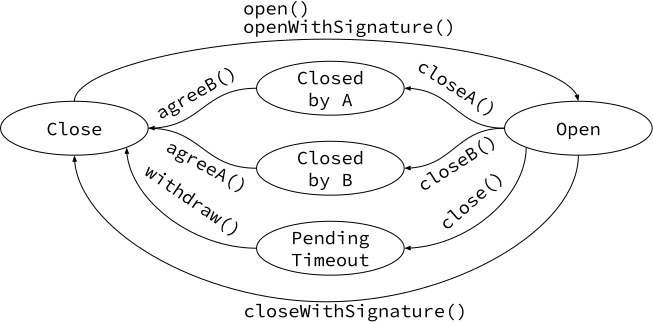
\includegraphics[width=\textwidth,keepaspectratio]{../yellowpaper/images/payment_channel_graph.png}
    \caption{Payment channel state graph}
    \label{fig:Payment channel graph}
\end{figure}

>>>>>>> 69f5d05030f54ccc0d062189db223fbd48a05cb5
\subsection{Proof Of Relay}

HOPR incentivizes packet transformation and delivery using a mechanism called “Proof-Of-Relay”.
This mechanism makes sure nodes relay services are verifiable.
\paragraph{Construction}
\begin{itemize}
    \item Every packet is sent together with a ticket.
    \item Each ticket contains a challenge.
    \item The validity of a ticket can only be checked on reception of the packet but the on-chain logic enforces a solution to the challenge stated in the ticket.
\end{itemize}
Since “Proof-Of-Relay” is used to make the relay services of nodes verifiable, it is the duty of each node to check that given challenges are derivable from the given and the expected information.
Packets with inappropriate challenges should be dropped as they might not lead to winning tickets.
Therefore, the sender of the packet also provides a hint of the expected value that a node is supposed to get from the next downstream node (as explained in the ticket section).










